% !TeX spellcheck = en_US
\chapter{Structured preferences}
\label{ch:structpref}

How can we use the concept introduced to choose a solution for a decision problem? 

We'll assume: 
\begin{itemize}
	\item A simple preference relation $\Pi$
	
	\item A certain environment $|\Omega| = 1 \implies f(x, \bar \omega)$ reduces to $f(x)$
	
	\item A single decision-maker $|D| = 1 \implies \Pi_d$ reduces to $\Pi$
\end{itemize}

Single scenario and single decision-maker. Also, the preference relation of the decision-maker will be a weak order (reflexive, transitive and complete).

The first two conditions allow a well-posed definition of solutions that can be justifiably selected and the third allows the choice of a single solution.

\section{Dominance relation}
\label{sec:dominancerel}

The preference relation between impacts $(\Pi \subseteq F \times F)$ projects onto an \textbf{induced relation between solutions}. A solution \textit{dominates} another when the impact of the former is preferable to the impact of the latter.
$$ x \wpref{} x' \Leftrightarrow f(x) \wpref{} f(x') \quad \forall x, x' \in X $$

\begin{definition}
	We denote as \textbf{dominated solution} a solution $x \in X$ such that $\exists x' \in X : f(x') \prec f(x)$, \textbf{nondominated solution}. We denote as $X^\ast \subseteq X$ the set of \textbf{all nondominated solutions}.
\end{definition}

This implies a partition of the feasible region into
\begin{itemize}
	\item dominated solutions: $x \in X$ such that $\exists x' \in X: x' \prec x$
	
	\item nondominated solutions: the other ones
\end{itemize}

\textbf{Reflexivity} looks natural in a preference relation. When solving a decision problem, it is also rather natural to 
\begin{itemize}
	\item \textbf{exclude dominated solutions}, that is choose $x^\ast \in X^\ast$
	
	\item Choose an \textbf{arbitrary solution from a set of mutually indifferent ones}
\end{itemize}

But this conflicts with some possible situations: 
\begin{itemize}
	\item All solutions in a strict dominance circuit would be removed
	
	\item Two solutions might be indifferent with respect to a third one, but incomparable with each other
\end{itemize}

Transitivity solves both problems. \textbf{Preorders} are strong candidates to \textbf{be preference relations}.

\subsection{Decision-making on preorders}
\label{subsec:decisionmakingpreorders}

\begin{theo}
	If the preference relation $\Pi$ is a preorder, the induced dominance is a preorder. \\
\end{theo}

\begin{theo}
	If the preference relation $\Pi$ is a preorder (reflexive and transitive) and the solution set is finite and nonempty ($X \neq \emptyset$), the nondominated solution set $X^\ast$ is nonempty.
\end{theo}

This guarantees that decision problems admit reasonable solutions. In some cases, $X^\ast$ will contain a single solution, or several mutually indifferent, in other cases it will include incomparable solutions. Therefore, determining $X^\ast$ simplifies the problem, but doesn't solve it completely.

\begin{theo}
	If preference $\Pi$ is a preorder and $X^\ast$ is nonempty, the nondominated solutions partition into disjoint components
	\begin{itemize}
		\item they are mutually indifferent within each component
		
		\item they are mutually incomparable between different components
	\end{itemize}
	$\implies$ if there is only one component, the problem is solved (requires completeness).
\end{theo}

\subsubsection{Identification of the nondominated solutions}

If $X$ is a finite set, it's possible to build the \textbf{strict preference graph}, whose nodes correspond to solutions, while the arcs correspond to solution pairs whose impacts are related by a strict preference. In this graph there are no indifferent pairs. 

The nondominated solutions correspond to \textit{nodes with no ingoing arc} (from each node there's an arrow towards dominated solutions), to identify them it's sufficient to scan each node of the graph and search for nodes with zero indegree.

Let $O(\gamma)$ be the complexity of computing the preference between two given impacts (non necessarily constant, they must be computed and compared), then the overall complexity for the search is $O\left(\gamma |X|^2\right)$ (for each node, compare its impact to the one ov every other in time $\gamma$).

This obviously can't be applied to infinite sets and could be impractical even in the case of combinatorial sets.

\subsection{Decision-making on weak orders}
\label{subsec:decisionmakingweakorders}

\begin{theo}
	If preference $\Pi$ is a weak order (reflexive, transitive and complete), the induced dominance is a weak order. \\
\end{theo}

\begin{theo}
	If preference $\Pi$ is a weak order (reflexive, transitive and complete) and $X$ is finite and nonempty, nondominated solutions exist and are all mutually indifferent.
\end{theo}

This allows to choose any of such solutions as the overall solution of the problem. This is good, the aim is to "make the right choice". Weak orders allow to sort impact on a line, with possible ties, as if associating a degree to each impact.

\begin{definition}
	A \textbf{value function} is a function $v: F \rightarrow \R$ that associates a real value to each impact (also called \textit{utility functions in economics}). Function $v$ is \textbf{consistent} with preference relation $\Pi$ when 
	$$ f \wpref{} f' \Leftrightarrow v(f) \geq v(f'), \quad \forall f,f' \in F$$
	or, equivalently
	$$ \Pi = \left\{(f, f') \in F \times F \mid v(f) \geq v(f') \right\} $$
\end{definition}

This offers a compact way to represent preference relations, that is also good for computation
$$ \max_{x \in X} \left\{ v\left(f(x)\right) \right\}$$
if we have analytic expressions for $X$ and $v\left( f (\cdot)\right)$ and a solving algorithm.

Value functions are \textbf{not univocal} (infinite equivalent ones always exist).

If a preference relation admits a consistent value function, the derived relations of indifference and strict preference correspond to identity and strict inequality between the values of the value function. \\

\begin{theo}
	If a preference relation $\Pi$ admits a consistent value function $v(f)$, then $\Pi$ is a weak order (reflexive, transitive and complete).
\end{theo}

The proof is simple, the point is to show that the preference enjoys reflexivity (because $\Pi$ includes pair $(f,f)$ for all $f \in F$), transitivity (because for all triplets $f, f', f'' \in F$ such that relation $\Pi$ includes pairs $(f,f')$ and $(f', f'')$, it also includes pair $(f, f'')$), and completeness (because for each pair $(f, f')$ not included in $\Pi$, pair $(f',f)$ belongs to it).
%TODO: proof is missing, maybe do it?

In practice, we start from a preference relation, not from a value function, the inverse would be more useful (the decision problem could be reduced to a maximization of the value function), but it's not always true.

\subsubsection{Weak orders not reducible to a consistent value function}

\paragraph{Lexicographic order} The main example of weak order relation (actually, strong order relation), which doesn't admit a consistent value function. 

Considering the simplest two-dimensional case, with real components ($F = \R^2$), the preference relation is defined as
$$ 
\left[
\begin{array}{c}
	f_1 \\
	f_2
\end{array}
\right] \wpref{}  \left[
\begin{array}{c}
	f_1' \\
	f_2'
\end{array}
\right]
\Leftrightarrow f_1 < f_1' \text{ or } f_1 = f_1' \wedge f_2 \leq f_2'
$$
The decision-maker prefers the smaller impact of the first one, for any value of the second, preferring the smaller value of the second only in the case of a tie for the first.

It can be proven that this relation doesn't admit any consistent value function $v(f)$, that is assigning to each impact in $F$ a real value such that the preference between two impacts correspond to an inequality between the function values.

The intuitive reason is that no improvement of the second can compensate for a worsening, even very small, of the first.

\subsubsection{Multiplicity of the consistent value functions}
\label{subsubsec:multeplicityvalfunc}

The existence of a way to build a consistent value function does not imply its uniqueness. \\

\begin{theo}
	Given a value function $v: F \rightarrow \R$, consistent with a preference relation $\Pi$ on $F$, for any strictly increasing function $\phi: \R \rightarrow \R$ the composite function $\phi(v(\cdot))$ is also consistent with $\Pi$.
\end{theo}

If a weak order admits a consistent value function, it admits infinite equivalent ones, that associate to the same impacts different values, but sorted in the same way.

%P78 notes, section not part of the syllabus, read it and weep

\subsubsection{Weak order preference models}

\paragraph{Scalar impact} When the impact is one-dimensional, it's often easy (though not always) to turn it into a value function. E.g., if the impact
\begin{itemize}
	\item is a benefit, set $v(f) = f$
	
	\item is a cost, set $v(f) = -f$
	
	\item has a target value $\bar f$, set $v(f) = - \dist(f, \bar f)$
\end{itemize}

\paragraph{Borda count} In the finite case, every weak order admits a value function (Borda count)
$$ B(f) = |\left\{f' \in F \mid f \wpref{} f' \right\}|$$

Basically, the Borda count $B(f)$ is the number of solutions dominated by $f$.

\paragraph{Lexicographic order} If the indicators are all costs (or benefits) and are sorted by importance ($P = (\pi_1, \dots, \pi_p)$), the preference relation $\Pi$ is a total order
$$ f \wpref{} f' \Leftrightarrow f_{\pi_1} < f_{\pi_1}' \text{ or } \left\{
\begin{array}{c}
	f_{\pi_1} = f_{\pi_1}' \\
	f_{\pi_2} < f_{\pi_2}' 
\end{array}\right\} \text{ or } \dots \text{ or } \left\{\begin{array}{c}
f_{\pi_1} = f_{\pi_1}' \\
f_{\pi_2} = f_{\pi_2}'  \\
\dots  \\
f_{\pi_p} \leq f_{\pi_p}'
\end{array}\right\}
$$

It does not admit value functions, but can be solved as follows
\begin{itemize}
	\item find the whole set $X^\ast_{\pi_1}$ of optimal solutions for $\min_{x \in X} f_{\pi_1}(x)$
	
	\item find the whole set $X^\ast_{\pi_2}$ of optimal solutions for $\min_{x \in X^\ast_{\pi_1}} f_{\pi_2}(x)$
	
	\item \dots
	
	\item find a single optimal solution $x^\ast_{\pi_p}$ for $\min_{x \in X^\ast_{\pi_{p-1}}} f_{\pi_p}(x)$
\end{itemize}

\paragraph{Utopia point} This model of preference:
\begin{enumerate}
	\item Identifies an ideal impact $f^\ast$ independently optimizing each indicator
	$$ f_l^\ast = \min_{x \in X} f_l (x) $$
	and combining the optimal values in a vector $f^\ast = \left[f_1^\ast \dots f_p^\ast \right]^T$. Determining such value is a classical optimization problem, sometimes hard, but generally possible
	
	\item Finds a solution with impact having minimum "distance" from $f^\ast$
	$$ \min_{x \in X} \dist \left(f(x), f^\ast \right)$$
\end{enumerate}

Different definitions of distance imply different results (Manhattan distance, Euclidean distance, \dots; infinite different distances can be defined), and the choice is arbitrary. 

If the indicators are heterogeneous, the units of measure have an influence and conversion coefficients are required to standardize them. The choice of coefficient is complex and, at least partly, arbitrary.

%End L4

\section{Multi Attribute Utility Theory MAUT}
\label{sec:maut}

The \textbf{Multi Attribute Utility Theory (MAUT)} assumes that the preference relation of the decision-maker is a weak order, admitting a consistent value function, but the decision-maker is unable to make the value function explicit without help.

It poses the problem to derive from the preference relation $\Pi$ the consistent value function $u: F \rightarrow \R$. We'll denote $u(f)$ as \textit{utility function} (economical notation).

We assume: 
\begin{itemize}
	\item a preference relation $\Pi$ with a consistent utility function $u(f)$ 
	
	\item a certain environment: $|\Omega| = 1 \implies f(x, \bar \omega)$ reduces to $f(x)$
	
	\item a single decision maker: $|D| = 1 \implies \Pi_d$ reduces to $\Pi$
\end{itemize}

And we know the preference $\Pi$, but not the utility function $u(f)$. \textit{How to build it?}

Specific models of preference have specific applications, \textit{case by case, they might work or not}. We want a \textbf{general way to derive $u(f)$ from $\Pi$}
\begin{enumerate}
	\item Introduce a graphical tool (indifference map)
	
	\item Turn the graph into a function, with a complex error-prone process 
	
	\item Define a special case with a simpler process (additive value functions)
	
	\item Characterize the preference relations falling within the special case
\end{enumerate}


\subsection{Indifference Curves}
\label{subsec:indifferencecurves}

\begin{definition}
	Given an impact set $F$ in the space of the indicators $\R^p$ and a preference relation $\Pi$ which is a weak order, we denote as \textbf{indifference curve} every subset of impacts that are reciprocally different.
\end{definition}

An indifference curve is a set $I \subseteq F$ of \textbf{reciprocally indifferent impacts}. They always enjoy the following properties: 
\begin{itemize}
	\item The \textbf{curves covers} $F$: every impact belongs to a curve, due to the completeness of the relation
	
	\item Any two indifference curves $I$ and $I'$ have \textbf{empty intersection} (transitivity would merge them)
	
	\item The weak order on impacts maps onto a \textbf{total order on curves (antisymmetry)}; there are no incomparable impacts and all indifferent impacts belong to the same curve, so impacts on different curves are linked by strict preference
\end{itemize}

Usually, technical assumptions are made:
\begin{itemize}
	\item \textbf{Continuity} implies that the curves are \textit{regular mathematical objects} and not completely general set of points
	
	\item The utility function $u(f)$ has a \textbf{continuous infinity of values} $c \in \R$ 
	
	\item Each indifference curve is expressed in \textbf{implicit form}
	$$ u(f) = c $$
	
	\item When the implicit form $u(f) = c$ can be turned into an \textbf{explicit form}
	$$ f_l = f_l \left(c, f_1, \dots, f_{l-1}, f_{l+1}, \dots , f_p\right) $$
	an indifference curve is a \textbf{hypersurface of $p-1$ dimensions in $\R^p$} (when $p = 2$, it's a line in the plane)
\end{itemize}

If a value function is known, the family of all indifference curves admits an analytic representation in the indicator space $F$ through the equation $u(f) = c$, where $c$ is a constant parameter that identifies each single curve. This corresponds to an analytic representation of the solution space $X$ through the parametric equation $u(f(x)) = c$.

\subsubsection{Indifference curves and utility function (Indifference map)}

If a preference relation admits a consistent value function, it admits infinitely many (as seen in \ref{subsubsec:multeplicityvalfunc}); the indifference curves of such functions, however, are always the same. 

The correspondence between preference relations and indifference curves is one-to-one, the one between preference relations and value functions is one-to-many.

Given a weak order preference relation $\Pi$ on $F$, its \textbf{indifference map} $\I_\Pi$ is the ordered family of indifference curves covering $F$. The correspondence between $\Pi$ and $\I_\Pi$ is one to one
\begin{itemize}
	\item $\Pi$ identifies all groups of indifferent impacts (curves) and their order
	
	\item $\I_\Pi$ identifies the preference between all pairs of impacts
\end{itemize}

The indifference map $\I_\Pi$ corresponds to infinite utility functions $u(f)$.

\subsection{Determining the utility function}

Given a preference relation $\Pi$ on $F$: 
\begin{enumerate}
	\item Extract a sample $\tilde F$ from $F$
	
	\item Ask the decision-maker to 
	\begin{itemize}
		\item sort the sampled impacts
		
		\item Identify their equivalence classes
	\end{itemize}
	
	\item Draw an interpolating curve for each equivalence class 
	
	\item Guess a parametric utility function family from their shape 
	$$ u = u_\alpha (f) \text{ with } \alpha = \left[\alpha_1 \dots \alpha_p \right]^T $$
	
	\item Each pair of indifferent impacts implies an equation on $\alpha$
	$$ f \sim f' \Leftrightarrow u(f(\alpha)) = u(f'(\alpha)) $$
	
	\item Add a normalization condition to select one of the equivalent utilities
	
	\item Make consistency checks by comparing other pairs of impacts; if they fail, go back to 4 and change the parametric utility
\end{enumerate}

The process is, in general, very complex and error prone
\begin{itemize}
	\item Large samples are costly
	
	\item The sample must include at least $p-1$ pairs of indifferent impacts found by trial and error
	
	\item Small samples ($\approx p$) lead to likely incorrect curves; if the samples is too large, the workload for the decision maker becomes huge (if $k$ different values for each indicator leads to $k^p$ different impacts to evaluate)
	
	\item Numerical errors over many equations combine in cascade
	
	\item Mutually dependent pairs are useless
	
	\item High dimensional spaces make it hard to draw curves and guess $u_\alpha$
\end{itemize}

Some properties (not guaranteed) which allow to make easier estimates, helping to draw curves and guessing $u(f)$:
\begin{itemize}
	\item \textbf{Invertibility:} $u(f)= c$ can be solver with respect to each $f_l$
	\begin{itemize}
		\item always verified when the indicators are costs or benefits
		
		\item basically, when we can get each indicator $f_l$ from the function $u(f)$ (analytically, the function can be inverted)
	\end{itemize}
	Under this assumption, an indifference curve $u(f) = c$ can be written in explicit form as $f_l = f_l (c, f_1, \dots, f_p)$
	
	\item \textbf{Monotony:} strictly decreasing or increasing difference curves (\textit{an increase in one is balanced by a decrease in another})
	\begin{itemize}
		\item always verified when the indicators are all costs or benefits
	\end{itemize}
	In order to compensate for the variations of an indicator, the other ones must vary in a well-determined direction
	
	\item \textbf{Convexity} or \textbf{concavity} ("law of diminishing marginal utility"): 
	\begin{itemize}
		\item costs lead to concave curves, benefits to convex ones
	\end{itemize}
	The indifference curves compensate for the increase of an indicator by a certain amount with variations of the other ones that increase (or decrease) with the value of the first indicator; basically, if a resource (indicator) is scarce, increasing it brings a large utility, compensated by a strong decrease of other resources, if a resource is abundant the same increase brings a small utility, compensated bt a weak decrease of other resources (this is the case of convex curves, they would be concave in the case of indicators expressing cost)
\end{itemize}

\subsection{Additive utility functions (game changer)}

\begin{definition}
	We denote a utility function as \textbf{additive} when it can be expressed as the sum of functions of the single indicators:
	$$ u(f_1, \dots, f_p) = \sum_{l = 1}^p u_l (f_l) $$
\end{definition}

It's a specific case that brings many simplifications:
\begin{itemize}
	\item Ask different decision-makers for each indicator $f_l$ (\textit{split the work})
	
	\item Ask decision-makers with experience in the sector (\textit{more reliable})
	
	\item Compare scalar values $f_l$ instead of vectors $f$ (\textit{easier and better})
	
	\item Build functions $u_l (f_l)$ with one argument (\textit{easier and better})
\end{itemize}

Since a utility function has infinitely many forms, \textbf{a nonadditive function can have an additive equivalent form}, but \textit{that is not guaranteed, how can we know?}

Example (Cobb-Douglas functions):
$$ u(f) = \prod_{l=1}^{p} f_l^{\alpha_l} \text{ is equivalent to } u'(f) = \log u (f) = \sum_{l = 1}^p \alpha_l f_l $$

If the utility function is additive, the problem of estimating it can be reduced to the estimation of $p$ single-variable functions, making the process easier.

\subsection{Preferential Independence}
\label{subsec:preferentialindependence}

How to know that $\Pi$ admits an additive consistent utility function? Given the set of attribute indices $P = \left\{1, \dots, p\right\}$, focus on subset $L \subset P$; we can write that
$$ f = \left[
\begin{array}{c}
	f_L \\
	f_{P\setminus L}
\end{array}
\right]$$
where $f_L$ and $f_{P\setminus L}$ are the subvectors of impact $f$ corresponding, respectively, to the indicators of $L$ and $P \setminus L$ (we just divided the whole thing in two parts).\\

\begin{definition}
	A proper subset of indicators $L$ is \textbf{preferentially independent} from the complementary subset $P \setminus L$ when, given two impacts with identical values of the indicators in $P \setminus L$, the preference relation between them does not depend on such values:
	$$ 
	\left[
	\begin{array}{c}
		f_L \\
		\phi 
	\end{array}
	\right]
	\wpref{}
	\left[
	\begin{array}{c}
		f_L' \\
		\phi 
	\end{array}
	\right]
	\Leftrightarrow
	\left[
	\begin{array}{c}
		f_L \\
		\psi
	\end{array}
	\right]
	\wpref{}
	\left[
	\begin{array}{c}
		f_Lì \\
		\psi
	\end{array}
	\right]
	$$
	for all subvectors $\phi$, $\psi$, $f_L$, $f_L'$ such that the four impacts are in $F$:
	$$ 
	\left[
	\begin{array}{c}
		f_L \\ \phi
	\end{array}
	\right],
	\left[
	\begin{array}{c}
		f_L' \\ \phi
	\end{array}
	\right],
	\left[
	\begin{array}{c}
		f_L \\ \psi
	\end{array}
	\right],
	\left[
	\begin{array}{c}
		f_L' \\ \psi
	\end{array}
	\right] \in F
	$$
\end{definition}

Preferences between values in $L$ do not depend on the values out of $L$. 

For example: a cost is preferentially independent from all other indicators (the lower the better), but this is not true for a thermostat, at a certain humidity a lower temperature is better, at other ones, a higher temperature might be better.

Preferential independence is \textbf{not symmetric}:
$$L \text{ independent from } P\setminus L \centernot \implies P \setminus L \text{ independent from } L $$

Preferential independence \textbf{on single indicators does not imply independence on larger subsets}: 
$$ \left\{l\right\} \text{ independent from } P \setminus \{l\}, \ \forall l \in P \centernot \implies L \text{ independent from } P \setminus L, \forall L \subseteq P $$

\subsubsection{Mutual preferential independence}

Preferential independence of relation $\Pi$ and additivity of function $u(f)$ are strictly connected, even if not rigorously equivalent. \\

\begin{definition}
	We say that a problem enjoys \textbf{mutual preferential independence} when every proper subset of indicators $L \subset P$ is independent from its complement $P \setminus L$.
\end{definition}

Mutual preferential independence is a necessary condition for additivity.

The above definition requires to check every nonempty proper subset $P \subset L$: 
\begin{itemize}
	\item $2^p - 2$ subsets
	
	\item infinite 4-tuples of subimpacts (to sample) for each subset \\
\end{itemize}

\begin{theo}
	Mutual preferential independence holds if and only if, given $\bar l \in P$, every pair $L = \left\{l, \bar l \right\}$ is preferentially independent from $P \setminus L$ for all $l \in P \setminus \{\bar l\}$
\end{theo}

We need to check only $p-1$ pairs (\textit{but single indicators are not enough}). \\

\begin{theo}
	If $\Pi$ admits a consistent additive utility function $u(f)$, then $\Pi$ enjoys mutual preferential independence.
\end{theo}

To verify this is enough to apply the definition (for a more detailed proof, p.92 of the notes).

The problem is that the opposite is needed, we can verify mutual preferential independence and not additivity, as the utility function is always unknown, we need a sufficient condition. \\

\begin{theo}
	A decision problem with $p \geq 3$ indicators enjoying mutual preferential independence admits an additive utility function $u(f)$.
\end{theo}

Unfortunately, when $p=2$, mutual preferential independence is necessary but not sufficient for additivity, as it reduces to checking each indicator with respect to the other one.

% End L4, p 93/94 of the notes

\subsection{Marginal rate of substitution MRS}
\label{subsec:mrs}

To summarize, we know the preference $\Pi$, not the utility function $u(f)$ and the general process to find it is complex and error-prone. For additive functions it's much simpler, but is $u(f)$ additive?
\begin{itemize}
	\item for $p \geq 3$, mutual preferential independence $\Leftrightarrow$ additivity
	\item for $p = 2$, mutual preferential independence $\impliedby$ additivity
\end{itemize}

The problem lies in how the indifference curves behave in $F$; the missing condition to guarantee additivity concerns the steepness of the indifference curve. We need a measure of steepness.

The behavior of a curve is described by the relation between $f_1$ and $f_2$: from $f$, vary $f_1$ and update $f_2$ so as to remain on the indifference curve. \\

\begin{definition}
	We denote as \textbf{marginal rate of substitution (MRS)} of $f_1$ with $f_2$ in a given impact $f$ the limit 
	$$ \lambda_{12} (f) = \lim_{\delta f_1 \rightarrow 0} - \frac{\delta f_2 (f, \delta f_1)}{\delta f_1} $$
	where $\delta f_2 (f, \delta f_1)$ is such that $f + \left[\begin{array}{c}
		\delta f_1 \\ \delta f_2 (f, \delta f_1)
	\end{array}\right] \sim f$
\end{definition}

In other words, the MRS is the limits, for infinitesimal variations of $f_1$, of the ration between the variations of $f_2$ and $f_1$ that produces impacts indifferent with respect to $f$. The sign of the limit is reversed because it's often negative (e.g. when the two indicators are both costs or benefits).

In problems with more than two indicators, a marginal rate of substitution os defined for each pair of indicators, and is computed assuming that all other indicators remain constant.

The definition assumes to start from an impact $f$, slightly modifying the value of indicator $f_1$ and determining the corresponding variation of $f_2$ that allows to stay on the initial indifference curve.

Assuming that the indifference curves are regular arcs and representing them in parametric form (two functions of parameter $\alpha$, continuous up to the first derivative): 
$$
\begin{cases}
	f_1 = f_1 (\alpha) \\ f_2 = f_2 (\alpha)
\end{cases}
$$

The variations $\delta f_1$ and $\delta f_2$ used in the definition of $\lambda_{12}(f)$ correspond to a variation $\delta \alpha$ of the parameter, guaranteeing that the impact remains on the indifference curve and allowing us to express the MRS as
$$ \lambda_{12} (f) ? \lim_{\delta f_1 \rightarrow 0} - \frac{\delta f_2 (f, \delta f_1)}{\delta f_1} = \lim_{\delta \alpha \rightarrow 0} - \frac{f_2 (\alpha + \delta \alpha) - f_2 (\alpha)}{f_1 (\alpha + \delta \alpha) - f_1 (\alpha)} = - \frac{\frac{df_2}{d\alpha}}{\frac{d f_1}{d \alpha}} $$

This form is useful to prove \textbf{reciprocity}:
$$ \lambda_{12} (f) = \frac{1}{\lambda_{21} (f)} $$

\paragraph{MRS and utility function} A second expression shows the relation between MRS and $u(f)$; by changing $\alpha$ we move along the indifference curve, but the utility function remains constant: $u(f(\alpha)) = c$ for all $\alpha$, therefore having a first derivative equal to zero with respect to $\alpha$:
$$ \frac{d u(f_1 (\alpha), f_2 (\alpha))}{d \alpha} = 0 \implies \frac{\partial u}{\partial f_1} \frac{d f_1}{d \alpha} + \frac{\partial u}{\partial f_2} \frac{d f_2}{d \alpha} = 0 \implies - \frac{\frac{df_2}{d\alpha}}{\frac{df_1}{d \alpha}} = \frac{\frac{\partial u}{\partial f_1}}{\frac{\partial u}{\partial f_2}} $$

And this implies that
$$ \lambda_{12} (f) = \frac{\frac{\partial u}{\partial f_1}}{\frac{\partial u}{\partial f_2}} $$

The MRS of $f_1$ with $f_2$ is the ratio of the partial derivatives of the utility function with respect to $f_1$ and $f_2$. If the utility depends strongly on $f_1$ and weakly on $f_2$, the MRS is large, i.e., a large variation of $f_2$ is required to compensate for a small variation of $f_1$.

This form also holds for $p \geq 3$ indicators, given that the rate of substitution is defined keeping all indicators constant, except for two.

\paragraph{MRS and indifference curves} If the indifference curves are invertible, each value of parameter $\alpha$ corresponds to a different value of $f_1$ and $f_2$, one can define  a function $\alpha = \alpha (f_1)$ which implies an explicit expression for the indifference curve: $f_2 = f_2 (\alpha (f_1))$. The first derivative of that expression is
$$ \frac{df_2}{df_1} = \frac{df_2}{d\alpha} \frac{d \alpha}{d_f1}  = \frac{\frac{df_2}{d\alpha}}{\frac{df_1}{d \alpha}} $$
From which
$$ \lambda_{12} (f) = - \frac{d f_2}{d f_1} $$

The MRS is the \textit{negative slope of the tangent to the indifference curve}; the steepness of the indifference curves, with a reverse sign.

In simple terms, the MRS is how much of $f_2$ are you willing to give away for a small increase of $f_1$.

\subsection{Additivity and MRS}
\label{subsec:additivityandMRS}

By combining two distinct values for $f_1$ ($f_1'$ and $f_1''$) and $f_2$ ($f_2'$ and $f_2''$) one can build four different impacts. In general, the  MRS in these four are fully independents, however, they can be related. \\

\begin{definition}
	We denote as \textbf{corresponding trade-off condition} the following property
	$$ \lambda_{12} (f_1', f_2') \lambda_{12} (f_1'', f_2'') = \lambda_{12} (f_1'', f_2') \lambda_{12} (f_1', f_2'') $$
	for every quadruplets of impacts $(f_1', f_2'), (f_1'', f_2''), (f_1'', f_2'),  (f_1', f_2'') \in F$.
\end{definition}

Some indifference maps enjoy such property, and it is \textbf{global}: it relates far away impacts.

The corresponding trade-off condition is easier to interpret if rewritten as
$$ 
\frac{\lambda_{12} (f_1', f_2')}{\lambda_{12} (f_1'', f_2')} = \frac{\lambda_{12} (f_1', f_2'')}{\lambda_{12} (f_1'', f_2'')}
\ \text{ or } \
\frac{\lambda_{12} (f_1', f_2')}{\lambda_{12} (f_1', f_2'')} = \frac{\lambda_{12} (f_1'', f_2')}{\lambda_{12} (f_1'', f_2'')}
$$

Basically, multiplying two MRSs on the diagonal of a rectangle (composed by 2 values for each of the 2 indicators) is the same as multiplying the two MRSs for the values on the opposite diagonal.

\begin{center}
	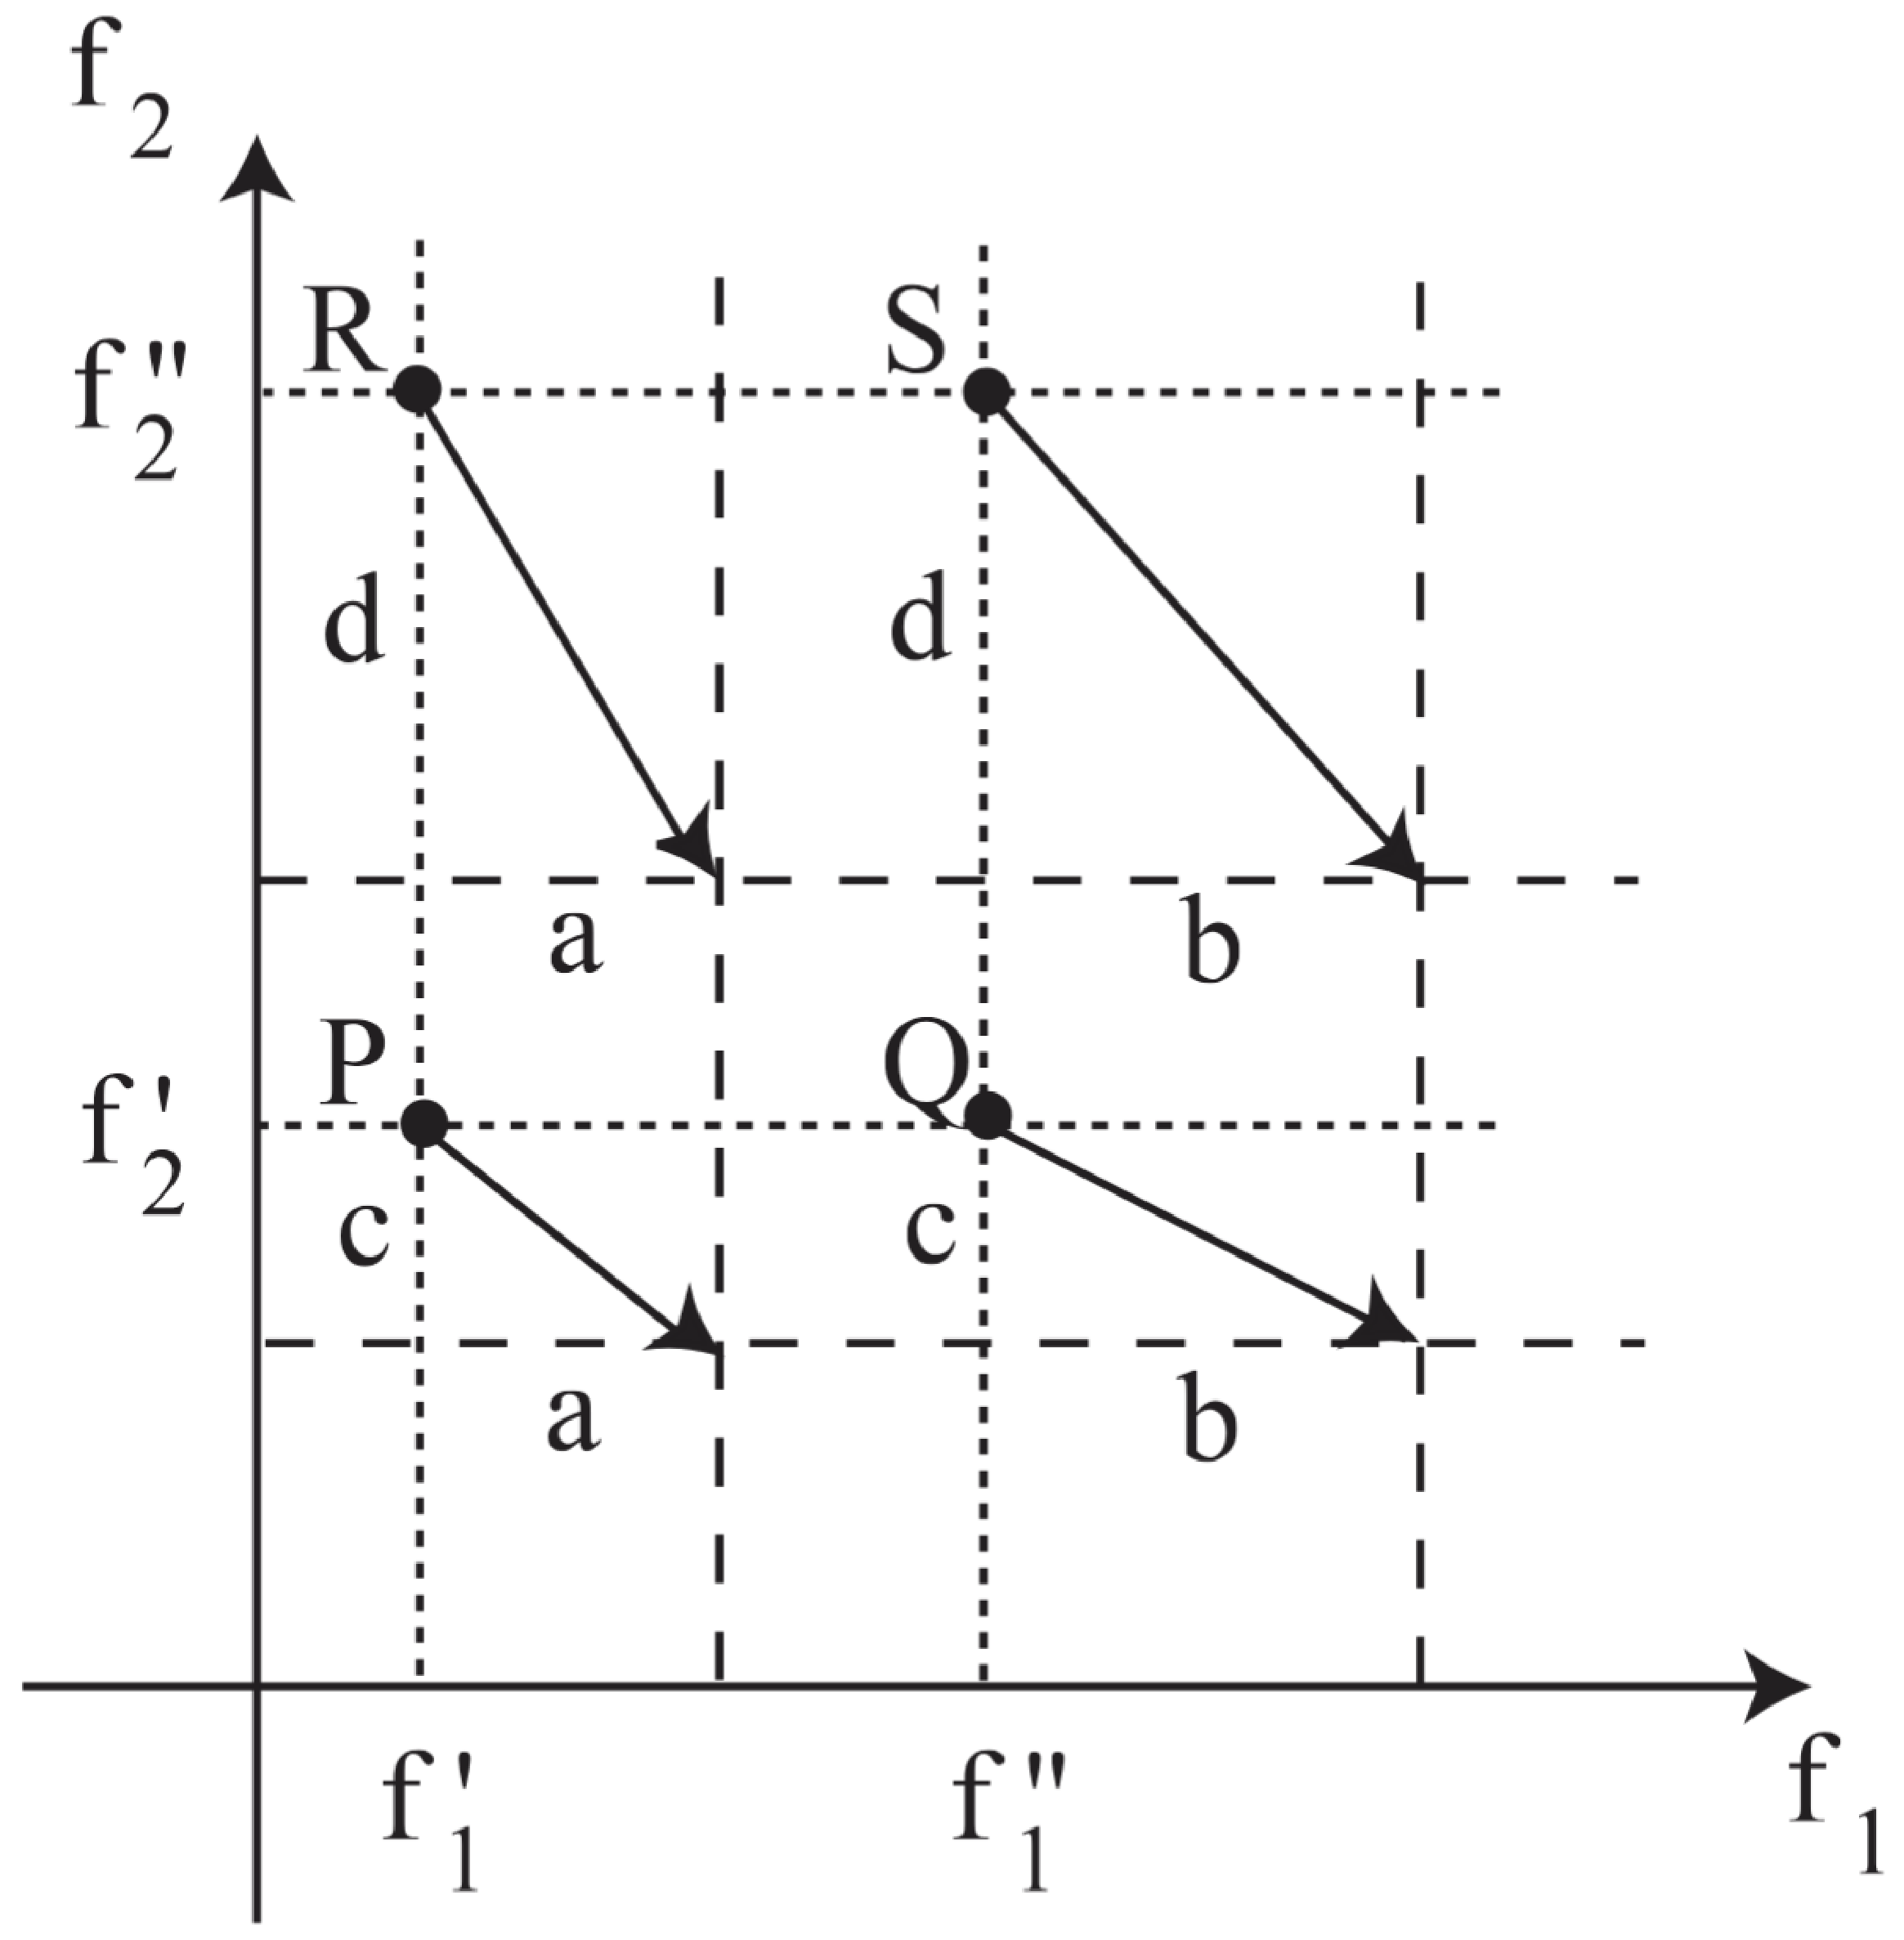
\includegraphics[width=0.45\columnwidth]{img/bdm/structpref/mrs1}
\end{center}
In the image it can be seen that in the four points $P$, $Q$, $R$ and $S$ the MRSs are, respectively, equal to $-a/c$, $-b/c$, $-a/d$, $-b/d$. The product of the rates in $P$ and $S$ is $ab/cd$, and it coincides with the product of the rates in $Q$ and $R$.

The ratio of $\lambda$ between points with the same abscissa does not depend on the abscissa. In other words, even if the MRS is nonuniform, it changes by the same factor moving between the same coordinates. \\

\begin{theo}
	A preference relation $\Pi$ admits an additive utility function $u(f)$ if and only if it enjoys both
	\begin{enumerate}
		\item mutual preferential independence
		
		\item the corresponding trade-off condition
	\end{enumerate}
\end{theo}

The "only-if part" it's easy to prove, the "if" was needed in order to assume additivity.

\begin{proof}
	Once again, it's a matter of applying the definition:
	$$ \lambda_{12} (f_1', f_2') \lambda_{12} (f_1'', f_2'') = \frac{\frac{\partial u}{\partial f_1'}}{\frac{\partial u}{\partial f_2'}} \frac{\frac{\partial u}{\partial f_1''}}{\frac{\partial u}{\partial f_2''}} $$
	Since $u(f_1, f_2) = u_1(f_1) + u_2(f_2)$:
	$$ \lambda_{12} (f_1', f_2') \lambda_{12} (f_1'', f_2'') = \frac{\frac{\partial u}{\partial f_1'}}{\frac{\partial u}{\partial f_2'}} \cdot \frac{\frac{\partial u}{\partial f_1''}}{\frac{\partial u}{\partial f_2''}} 
	= 
	\frac{\frac{\partial u}{\partial f_1'}}{\frac{\partial u}{\partial f_2''}} \frac{\frac{\partial u}{\partial f_1''}}{\frac{\partial u}{\partial f_2'}}
	$$
	and getting back to function $u(f_1, f_2)$:
	$$ 
	\lambda_{12} (f_1', f_2') \lambda_{12} (f_1'', f_2'') = \frac{\frac{\partial u}{\partial f_1'}}{\frac{\partial u}{\partial f_2''}} \frac{\frac{\partial u}{\partial f_1''}}{\frac{\partial u}{\partial f_2'}}
	= \lambda_{12} (f_1', f_2'') \lambda_{12} (f_1'', f_2')
	$$
\end{proof}

The corresponding trade-off condition is thus necessary for additivity (also sufficient, under suitable conditions).

To assume additivity: 
\begin{itemize}
	\item When $p \geq 3$, check mutual preferential independence for $p-1$ indicator pairs
	
	\item When $p=2$ check
	\begin{itemize}
		\item independence for the single indicators
		
		\item the corresponding trade-off condition
	\end{itemize}
\end{itemize}

\subsection{Building an additive utility function}
\label{subsec:buildingadditive}

The expression for an additive utility function
$$ u(f) = \sum_{l = 1}^p u_l (f_l) $$
assumes the same measure unit for all $u_l$ function. In practice, different fields use different units, therefore:
\begin{enumerate}
	\item Adopt normalized utilities: pure numbers $\tilde u_l (f_l)$ instead of $u_l (f_l)$, usually within the interval $[0,1]$
	
	\item Introduce weights $w_l$ to combine them
	$$ u(f) = \sum_{l = 1}^p w_l \tilde u_l (f_l) $$
\end{enumerate}

Intuitively, we are splitting the task into "rescaling" indicators into utilities, removing nonlinearities, and "combining" heterogeneous utilities into a single one.

The normalized utility expression is a \textbf{linear} and \textbf{convex} combination: 
\begin{itemize}
	\item \textbf{Conic:} all coefficients are nonnegative ($w_l \geq 0$ for all $l \in P$)
	
	\item \textbf{Affine:} the coefficients have unitary sum ($\sum_{l = 1}^p w_l = 1$)
\end{itemize}

\subsubsection{The bisection method}

Building a utility function for a one-dimensional impact ($F \subseteq \R$) is much easier than for a multidimensional one, it only takes comparing pairs of numbers and wondering which one of the two is better. 

However, the function we want to build must respect a condition stronger than just sorting all impacts, we want to measure the strength of relative preference: nearly indifferent impacts should have similar utility values and impacts well distinguished from a preferential point of view should have very different utility values.

The bisection methods builds such function with a dichotomic approach. For example, to build the normalized utility $\tilde u_C(C)$ for the daily calorie intake $C$, given $F_C = [0, 10000]$, interview an expert about a specific individual
\begin{enumerate}
	\item Ask the expert for the worst values in $F_C$ (for example, $C_1^\dag \leq 1000$ and $C_2^\dag \geq 6000$) and set $\tilde u_C (C) = 0$ for such values
	
	\item Ask the expert for the best values in $F_C$ (for example, $2200 \leq C^\ast \leq 2600$) and set $\tilde u_T (22) = 1$ for such values
	
	\item Ask the expert for values of exactly intermediate utility between $T^\dag$ and $T^\ast$ (for example, $C = 1800$ and $3000$) and set $\tilde u_C (C) = 1/2$
	
	\item Go on, asking for values of intermediate utility between the fixed ones and set $\tilde u_T$ accordingly
	
	\item Guess an interpolating function
\end{enumerate}

When the indicator represents a cost or benefit, sometimes it's possible to assume the utility proportional to the indicator $f_l$. We can easily generate a normalized utility function:
$$ \tilde u_l (f_l) = \frac{f_l - \min_{x \in X} f_l (x)}{\max_{x \in X} f_l (x) - \min_{x \in X} f_l (x)} $$
Switch them for costs.

If $\min_{x \in X} f_l (x)$ or $\max_{x \in X} f_l (x)$ are unknown or hard to compute, an underestimate and overestimate can be used instead, yielding a normalized utility function, different from above mentioned one. This can lead to a "compression" of the value range if the estimates are loose (it's not using the whole interval $[0,1]$).

\subsection{Determining the weights}

We still need to determine the weights with which to combine the components of the additive utility function. This requires to identify a sufficient number of pairs of indifferent impacts, equaling the utilities of the two impacts imposes a constraint on the weights of $w_l$, allowing us to find a single solution, with enough constraints (linear equation system).

As in the general case, $p-1$ independent pairs of indifferent impacts are needed: 
\begin{itemize}
	\item The equations are linear in $w$ 
	$$ f \sim f' \Leftrightarrow \tilde u (f) = \tilde u (f') \Leftrightarrow \sum_{l = 1}^p \tilde u_l (f_l) w_l = \sum_{l = 1}^p \tilde u_l (f_l') w_l$$
	
	\item The normalization condition imposes convexity 
	$$ \sum_{l = 1}^p w_l = 1$$
\end{itemize}

This process works correctly in the ideal case, but if indifference is imprecise, the pairs five wrong weights. The solution is to build a complete pairwise comparison of all indicators and analyze its consistency.

\subsubsection{The pairwise comparison matrix}

Select a pair of indifferent impacts $(f, f')$ with:
\begin{itemize}
	\item Different values for $f_l$ and $f_m$
	
	\item Identical values for all other indicators, $f_n = f_n'$ for all $n \in P \setminus \{l, m\}$
\end{itemize}

The equation reduces to 
$$ w_l \tilde u_l (f_l) + w_m \tilde u_m (f_m) = w_l \tilde u_l (f_l') + w_m \tilde u_m (f_m') $$
That simply becomes
$$ \tilde \lambda_{lm} = \frac{w_l}{w_m} = - \frac{\tilde u_m (f_m') - \tilde u_m (f_m)}{\tilde u_l (f_l') - \tilde u_l (f_l)} $$

\begin{definition}
	We denote as \textbf{pairwise comparison matrix} $\tilde \Lambda = \{\tilde \lambda_{lm}\}$ the matrix reporting all rates of substitution between the normalized utilities.
\end{definition}

It contains all the weight ratios
$$ \tilde \Lambda = \left\{\frac{w_l}{w_m}\right\} $$
expressing the relative weights between the single normalized utilities, that is, indicators (once nonlinearities and units of measure are removed).

A correct pairwise comparison matrix $\tilde \Lambda$ enjoys the following properties:
\begin{itemize}
	\item \textbf{Positivity:} $\tilde \lambda_{lm} > 0$ for all $l,m \in P$
	
	\item \textbf{Reciprocity:} $\tilde \lambda_{lm} = \frac{1}{\tilde \lambda_{ml}}$ for all $l,m \in P$
	
	\item \textbf{Consistency:} $\tilde \lambda_{ln} = \tilde{ \lambda_{lm}} \tilde \lambda_{mn}$ for all $l,m,n \in P$
\end{itemize}
We can check these properties on $\tilde \Lambda$ to be sure that $u(f)$ makes sense.

\subsection{The process in summary}

In summary, the process to determine the utility function is composed of the following steps: 
\begin{enumerate}
	\item Interview the decision-maker in order to understand whether mutual preferential independence holds (ask to compare different pairs of indicators with the complementary subset)
	
	\item In the positive case, focus on each attribute, fixing the other ones to any value, and build a single-variable component of the utility function with a method respecting the entity of the relative preference gaps
	
	\item Determine the weights with which to combine such functions, sampling impacts until a sufficient number of pairs of indifferent impacts has been found
	
	\item Check \textit{a posteriori} that the obtained utility function is valid, testing it on impacts not used before
\end{enumerate}

In any moment, it can be necessary to go back to correct the single components of the utility or even rejecting the additivity assumption, in which case the whole process is invalidated.

%End L6, p115 notes, skipping excercises